Se realizó una introducción al entorno de trabajo en el laboratorio y a los equipos que seran utilizados durante los experimentos, se tratan los procedimientos para la seguridad personal y manero de los productos quimicos del laboratorio.

\textbf{\textcolor{azul50}{Normas Generales:}}

Se presentan las normativas a seguir para el trabajo en el laboratorio, entre ellas se especifica que:\\[-1cm]
\begin{itemize}
    \item[-] Utiliza una bata y guantes de plástico. \\[-.6cm]
    \item[-] Guarda tus prendas de abrigo y los objetos personales en un armario o taquilla.\\[-.6cm]
    \item[-] Ten siempre tus manos limpias y secas. Las heridad deben ser tratadas y selladas.\\[-.6cm]
    \item[-] No fumar, comar o beber en el laboratorio.\\[-.6cm]
    \item[-] Fíjarse en los signos de peligrosidad que aparecen en los frascos de los productos químicos.\\[-.6cm]
    \item[-] Lávarse las manos con jabón después de tocar cualquier producto químico.\\[-.6cm]
    \item[-] Si se salpica accidentalmente, lavar la zona afectada con agua abundante. Si se salpica la mesa, límpiarla con agua y sécala después con un paño.\\[-.6cm]
    \item[-] Todos los productos inflamables deben almacenarse en un lugar adecuado y separados de los ácidos, las bases y los reactivos oxidantes.\\[-.6cm]
    \item[-] Los ácidos y las bases fuertes han de manejarse con mucha precaución, ya que la mayoría son corrosivos.\\[-.6cm]
    \item[-] No dejer destapados los frascos ni aspirar su contenido.\\[-.6cm]
    \item[-] Al acabar la práctica, limpia y ordena el material utilizado.
\end{itemize}
\textbf{\textcolor{azul50}{Estación de emergencia y señalizaciones de peligrosidad:}}

Se presenta la estación de emergencia (ver Fig. \ref{fig1.1}a) con regadera de cuerpo completo y lavaojos de emergencia. Válvula de acero inoxidable para accionar el cabezal aspersor jalando el maneral. Charola lava ojos de acero inoxidable. Además se instruye sobre la necesidad de llevar guantes, tapa bocas y batas siempre que sea necesario.
     \begin{figure}
    %\centering
    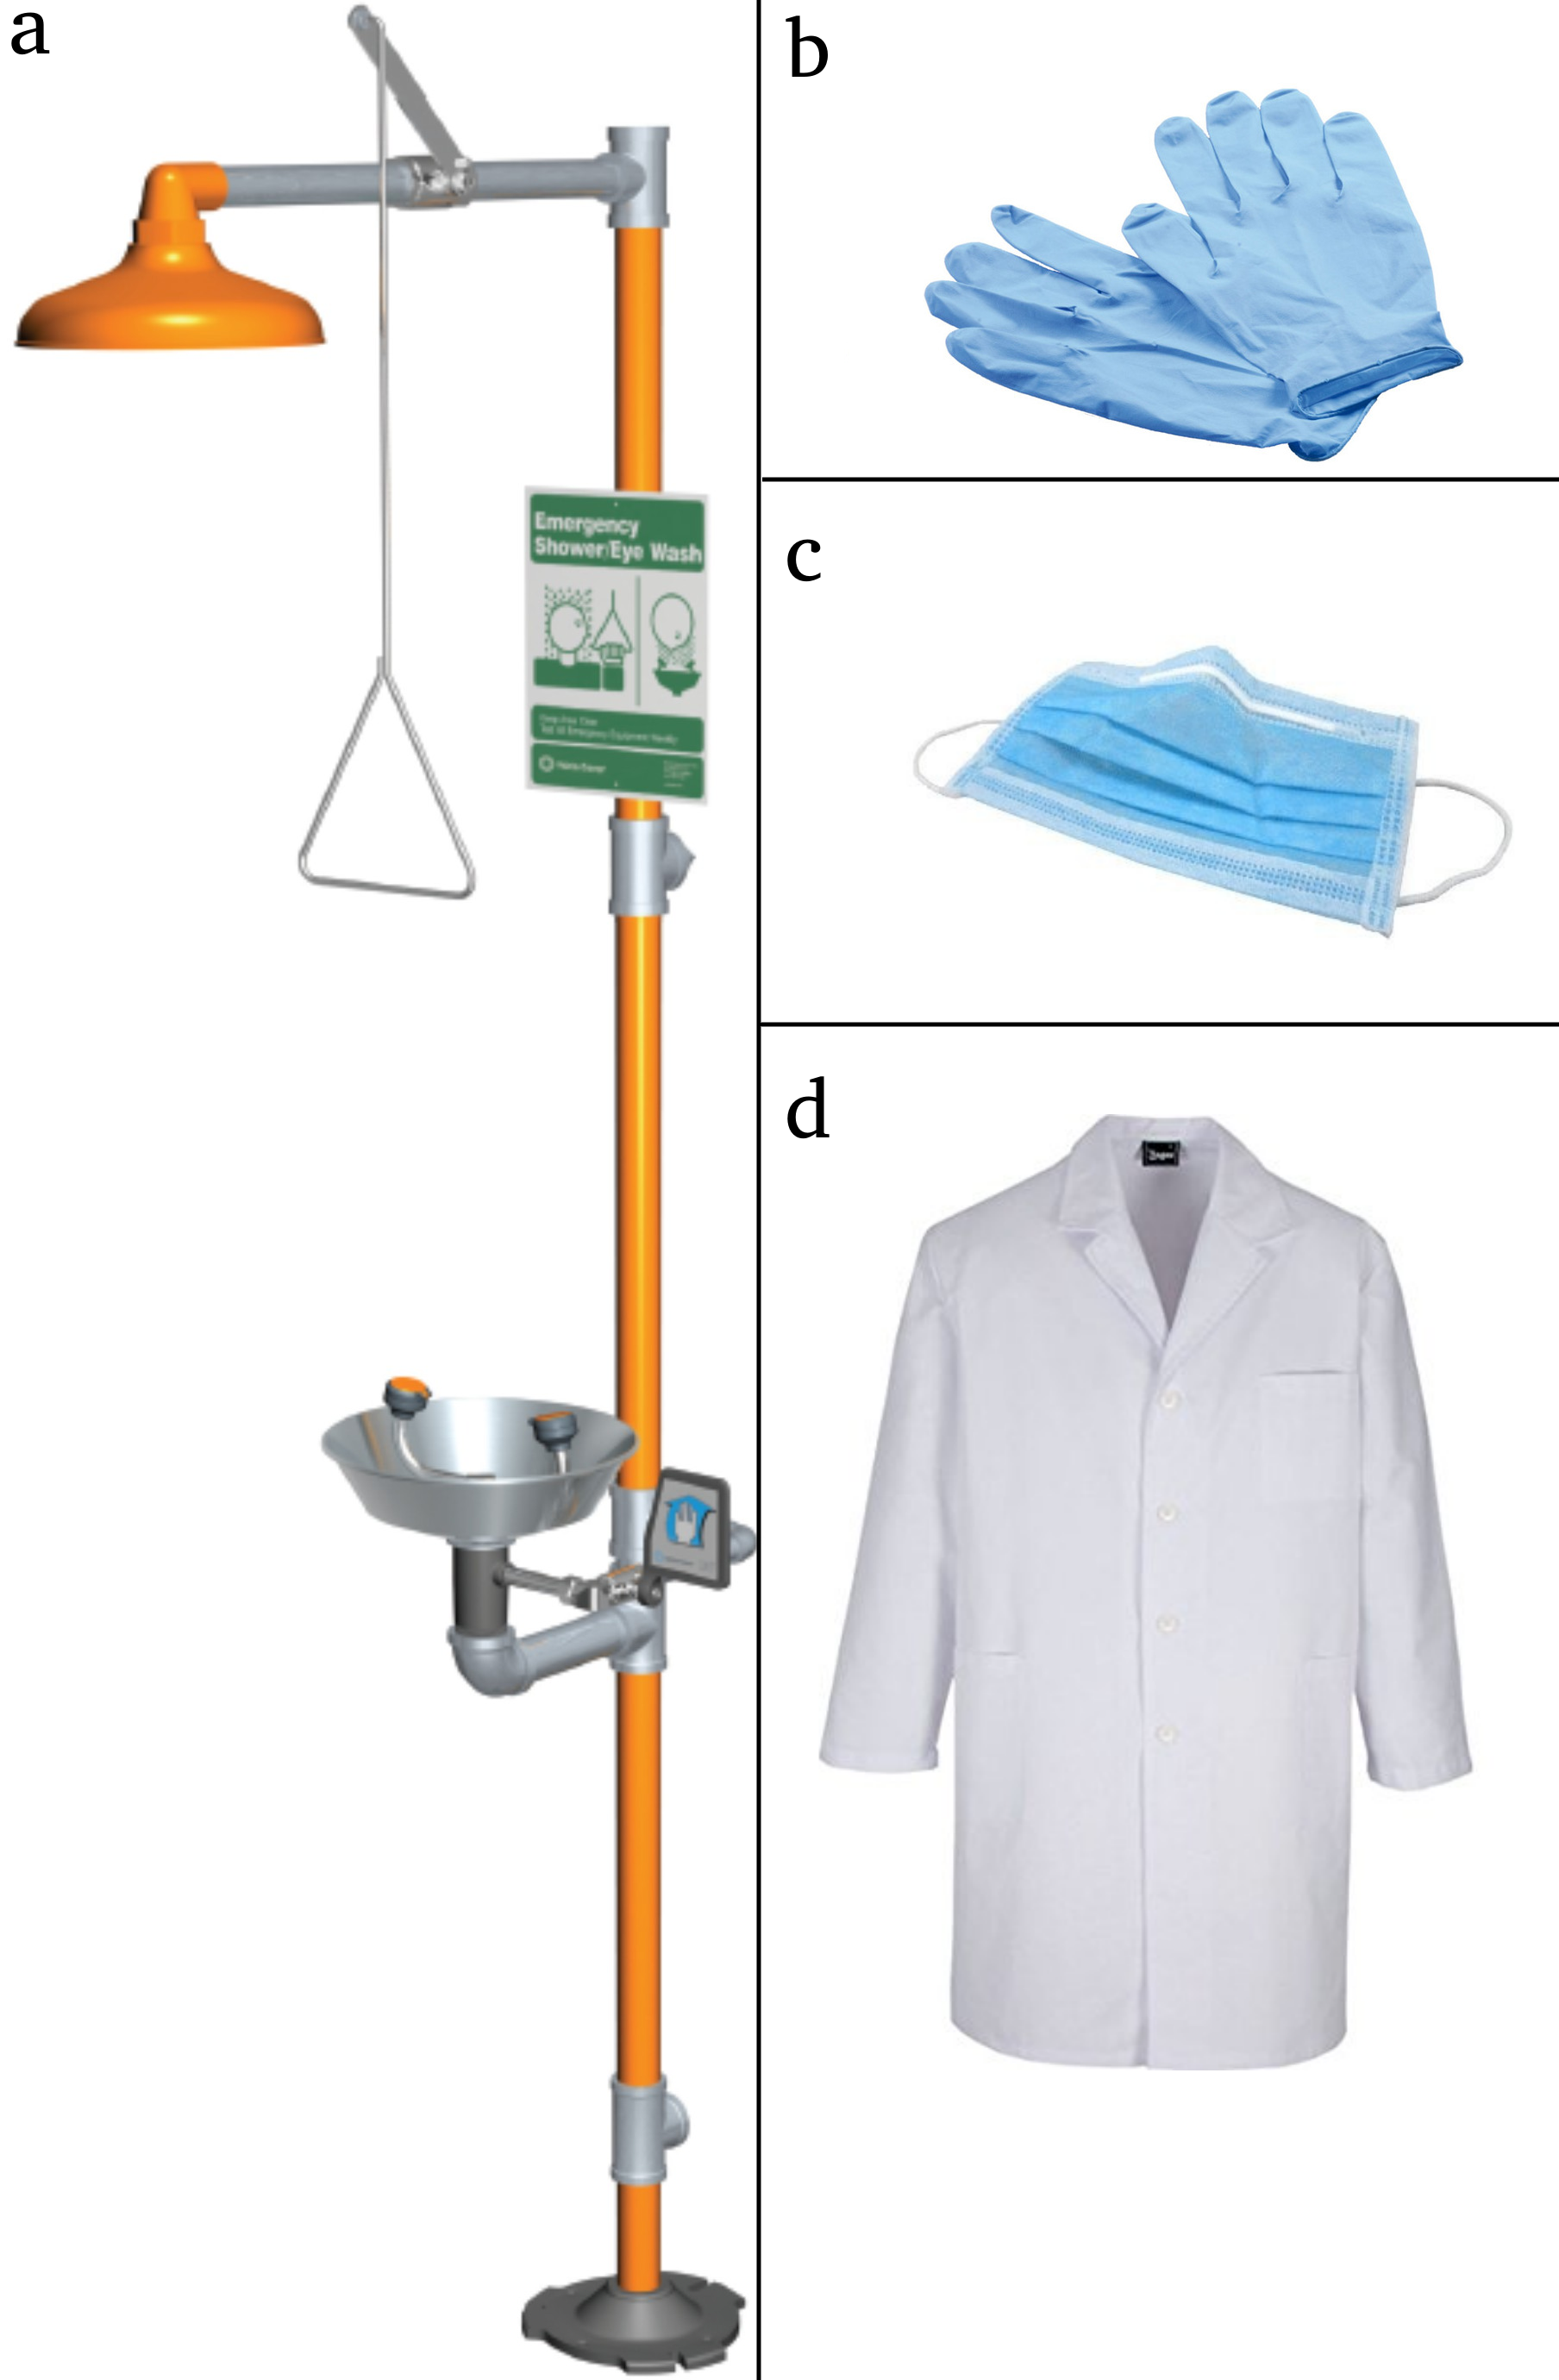
\includegraphics[width=0.4\textwidth]{Tarea1/emergencia.png}
    \caption{\textbf{Elementos de seguridad.}}
    \label{fig1.1}
    \end{figure}
Dada la naturaleza de los laboratorios a realizar, se necesita tener conocimientos de las señalizaciones de peligro que aparecen en los frascos, los mismos se muestran en la Fig. \ref{fig1.2}: 
\begin{figure}
    %\centering
    %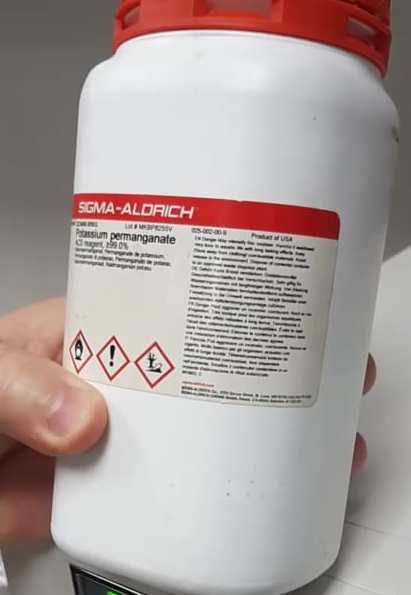
\includegraphics[width=0.3\textwidth]{Tarea1/muestras.png}
    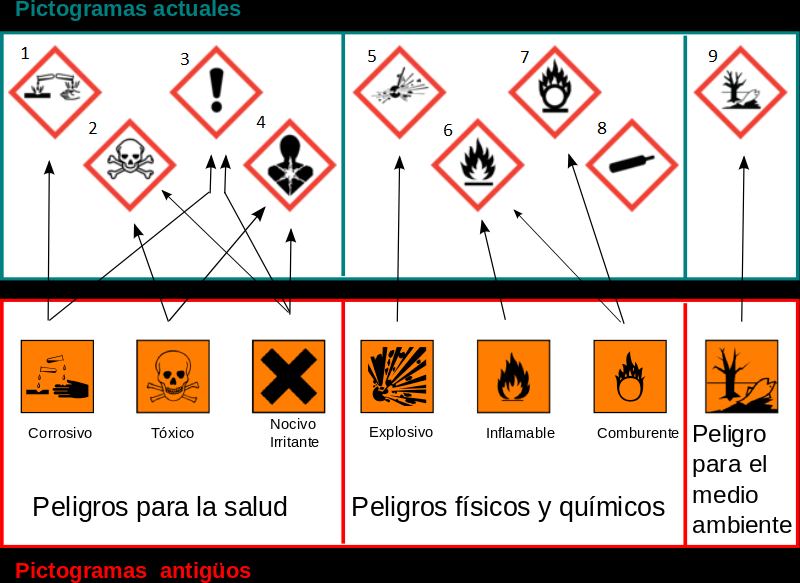
\includegraphics[width=0.44\textwidth]{Tarea1/toxico.png}
    \caption{\textbf{Pictogramas actuales y antiguos.}}
    \label{fig1.2}
\end{figure}
Guiandonos por los pictogramas de la Fig. \ref{fig1.2} podemos decir que:
\begin{itemize}
    \item[1)]  \textbf{\textcolor{morado}{Corrosivo}}: Estos productos químicos causan destrucción de tejidos vivos y/o materiales inertes. No inhalar y evitar el contacto con la piel, ojos y ropas.
    \item[2)]  \textbf{\textcolor{morado}{Tóxicidad aguda}}: Sustancias y preparaciones que por inhalación, ingesta o absorción a través de la piel, provoca graves problemas de salud e incluso la muerte. Todo el contacto con el cuerpo humano debe ser evitado. 
    \item[3)]  \textbf{\textcolor{morado}{Irritación cutánea}}: Clasificación: Sustancias y preparaciones que por penetración cutánea, pueden implicar riesgos graves, agudos o crónicos en la salud. Todo el contacto con el cuerpo humano debe ser evitado.
    \item[4)]  \textbf{\textcolor{morado}{Peligroso por aspiración}}: Sustancias y preparaciones que, por inhalación, ingestión o penetración cutánea, pueden implicar riesgos a la salud graves o agudos. Debe ser evitado el contacto con el cuerpo humano, así como la inhalación de los vapores. 
    \item[5)]  \textbf{\textcolor{morado}{Explosivo}}:Sustancias y preparaciones que pueden explotar bajo efecto de una llama o que son más sensibles a los choques o fricciones que el dinitrobenceno. Evitar golpes, sacudidas, fricción, flamas o fuentes de calor. 
    \item[6)]  \textbf{\textcolor{morado}{Inflamable}}: Sustancias y preparaciones que pueden calentarse y finalmente inflamarse en contacto con el aire a una temperatura normal sin necesidad de energía, o que pueden inflamarse fácilmente por una breve acción de una fuente de inflamación y que continúan ardiendo o consumiéndose después de haber apartado la fuente de inflamación, o inflamables en contacto con el aire a presión normal, o que, en contacto con el agua o el aire húmedo, emanan gases fácilmente inflamables en cantidades peligrosas. Evitar contacto con materiales ignitivos (aire, agua). 
    \item[7)]  \textbf{\textcolor{morado}{Comburente}}: Sustancias que tienen la capacidad de incendiar otras sustancias, facilitando la combustión e impidiendo el combate del fuego. Evitar su contacto con materiales combustibles. 
    \item[8)]  \textbf{\textcolor{morado}{Gas}}: Sustancias gaseosas comprimidas, líquidas o disueltas, contenidas a presión de 200 kPa o superior, en un recipiente que pueden explotar con el calor. No lanzarlas nunca al fuego.
    \item[9)]  \textbf{\textcolor{morado}{Peligroso para el medio ambiente}}: El contacto de esa sustancia con el medio ambiente puede provocar daños al ecosistema a corto o largo plazo. Debido a su riesgo potencial, no debe ser liberado en las cañerías, en el suelo o el medio ambiente. 
\end{itemize}
es bueno visualizar los pictogramas antiguos y como se relacionan con los modernos para evitar confusiones ante señalizaciones no actualizadas.

\textbf{\textcolor{azul50}{Instrumentaria en el laboratorio:}}

Tambien como parte de la introducción al laboratorio se hace una pequeña descripción del instrumental a utilizar durante toda la práctica, a continuación se realiza una descripción de ellos:
 \begin{itemize}
     %\item Balanza analitica.
     \item \textbf{\textbf{\textcolor{morado}{Balanza de Precision Series Pioneer Ohaus:}}} balanza diseñada para el pesaje de rutina básica en una variedad de aplicaciones de laboratorio, industrial y educación. Con la combinación correcta de rendimiento y funciones, la Pioneer de OHAUS ofrece un funcionamiento sin complicaciones para todas sus necesidades de pesaje. Posee un diseño compacto que permite que se adapte fácilmente en pequeñas áreas de mesas de laboratorio sin saturar el área de trabajo, con un indicador de nivel frontal superior ubicado al lado de la pantalla, ademas esta diseñada con ajustes de ambiente seleccionables y tres modos de filtro para garantizar operaciones precisas.%https://pesajeindustrial.com.pe/producto/balanza-de-precision-series-pioneer-ohaus/
     \begin{figure}
            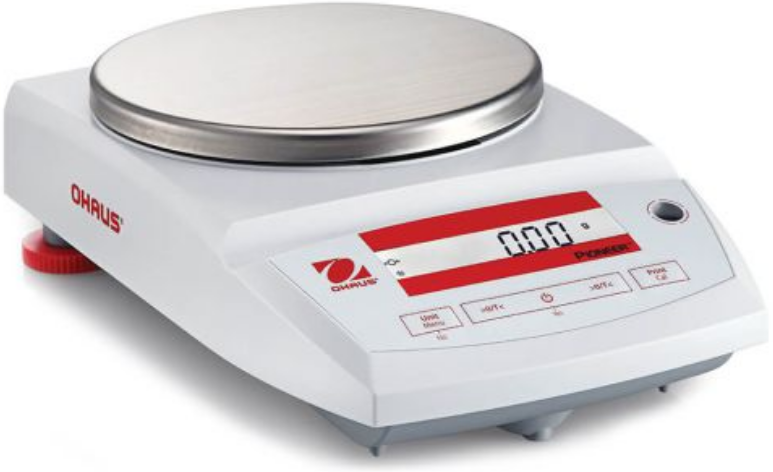
\includegraphics[width=0.4\textwidth]{Tarea1/balanza.png}
        \caption{\textbf{Balanza de Precision Series Pioneer Ohaus.}}
        \label{balanza}
    \end{figure}
     \item \textbf{\textbf{\textcolor{morado}{Incubador de Co2 MMM Linea CO2cell:}}} La línea CO2CELL es adecuada para la investigación y el crecimiento de cultivos celulares y de otro tipo, siendo muy frecuente su uso en el campo de la FIV. Un sistema de calentamiento de la cámara y la puerta único en el mercado elimina la necesidad de un ventilador, descartando así los riesgos de contaminación mutua de las muestras que con conllevan las vibraciones y la circulación forzada de la atmósfera de trabajo. La línea CO2CELL permite el trabajo en una atmósfera de CO2, eventualmente O2 i N2. El principio activo de la línea de incubadores CO2CELL está basado en el suave flujo gravitatorio del gas de operación en la cámara calefactada eléctricamente, con una alta humedad relativa y a la concentración de gas elegida.
     \begin{figure}
            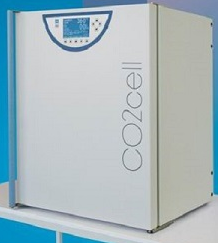
\includegraphics[width=0.4\textwidth]{Tarea1/cell.png}
        \caption{\textbf{Incubador de Co2 para crecimiento celular.}}
        \label{cell}
    \end{figure}
     \item \textbf{\textcolor{morado}{Analog Vortex Mixer}}:El mezclador de vórtice analógico proporciona modos de operación continua o táctil y control de velocidad variable. El diseño analógico permite una operación variable, desde una suave agitación con un arranque de bajas revoluciones hasta un vórtice vigoroso de muestras con capacidades de mezcla de alta velocidad. Este mezclador vortex es ideal en laboratorios de biociencia y otras aplicaciones. %https://www.laboratory-equipment.com/shakers-rotators/fisher-scientific-analog-vortex-mixer.php
     \begin{figure}
            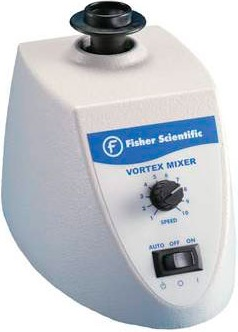
\includegraphics[width=0.2\textwidth]{Tarea1/agitador.jpg}
        \caption{\textbf{Analog Vortex Mixer.}}
        \label{agitador}
        \end{figure}
     \item \textbf{\textcolor{morado}{Logic Plus A2 con Purifier Logic+ Class II, Type A2 Biosafety Cabinets}}: son gabinetes de bioseguridad que brindan proteccion al producto y al medio ambiente contra partículas peligrosas. Tiene otras aplicaciones apropiadas incluyen el trabajo con medicamentos antineoplásicos, material genético, asbesto y sustancias adicionales que generan partículas peligrosas en el aire. %https://www.labconco.com/product/purifier-logic-class-ii-type-a2-biosafety-cabinets-2/4261
         \begin{figure}
            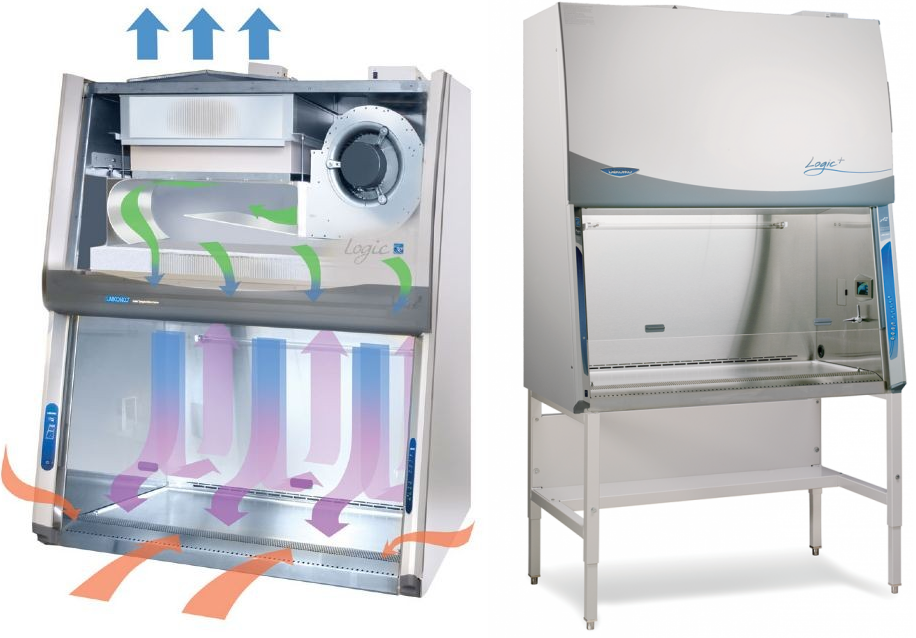
\includegraphics[width=0.44\textwidth]{Tarea1/cabina.png}
        \caption{\textbf{Thermo Scientific Heraeus Megafuge 16.}}
        \label{cabina}
        \end{figure}
     \item \textbf{\textcolor{morado}{Thermo Scientific Heraeus Megafuge 16}}: centrifugadora, la misma es perfecta para protocolos clínicos, aplicaciones de cultivo celular y procesamiento de microplaca, además de estar concebida para procesar muestras sensibles a la temperatura entre $-10^oC$ y $40^oC$ y poseen una capacidad de $4 \times 400~mL$. %https://www.thermofisher.com/order/catalog/product/75004230
         \begin{figure}
            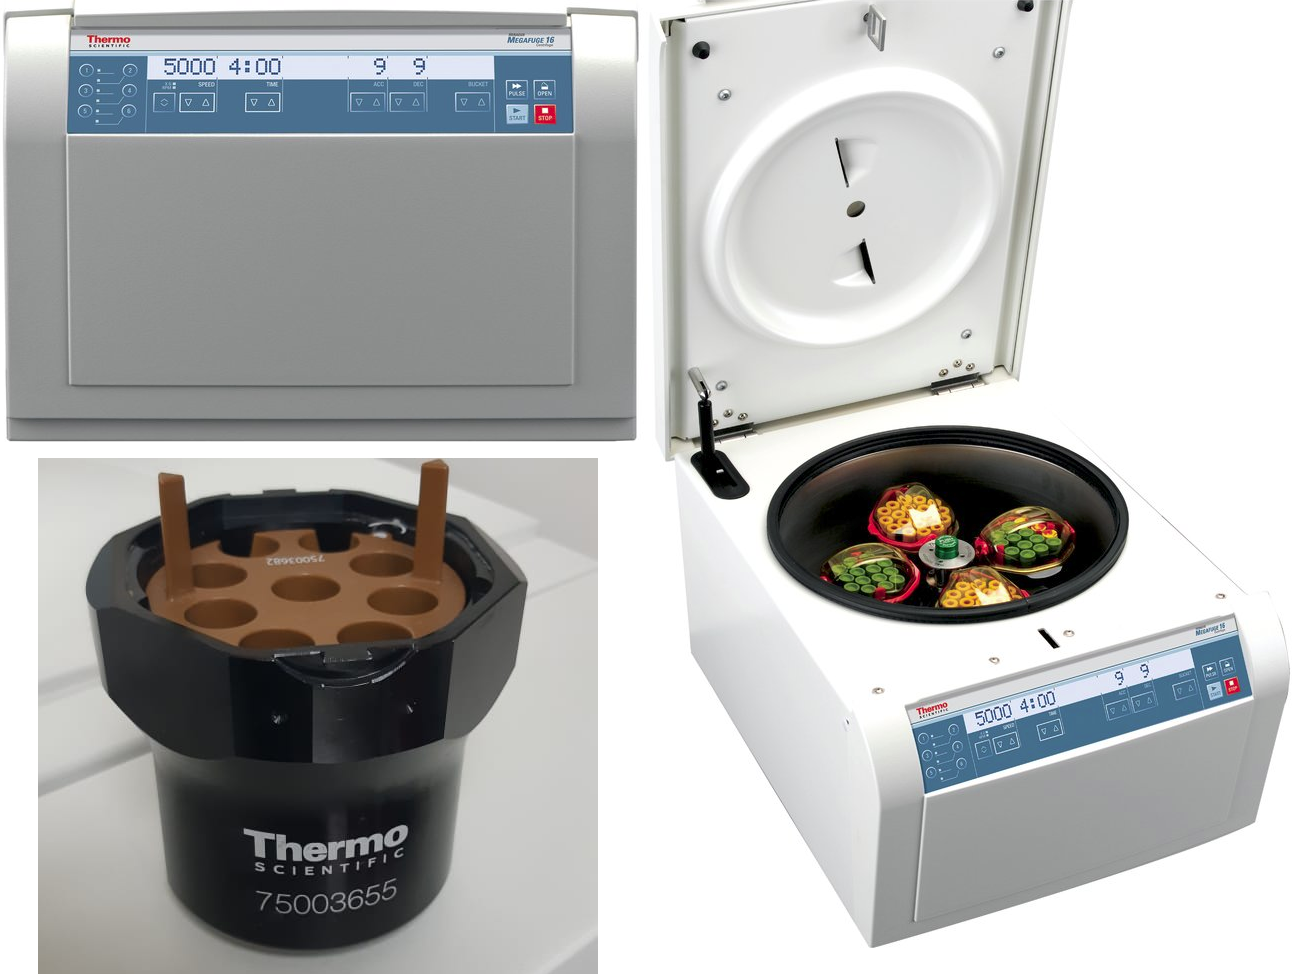
\includegraphics[width=0.44\textwidth]{Tarea1/centrifuga.png}
        \caption{\textbf{Thermo Scientific Heraeus Megafuge 16.}}
        \label{centrifuga}
        \end{figure}
     \item \textbf{\textcolor{morado}{Agitador RCT basic}}: es un agitador magnético IKA, con control de temperatura adicional para el modo más rápido de calefacción del medio sin supervisión, permite el ajuste del límite de temperatura por seguridad. Posee un circuito de seguridad ajustable de temperatura de la placa calefactora (50 - 360 °C). Además incluye un agitador magnético con calefacción seguro . %\textbf{https://www.ika.com/es/Productos-Lab-Eq/Agitadores-Magneticos-csp-188/RCT-basic-cpdt-3810000/
         \begin{figure}
            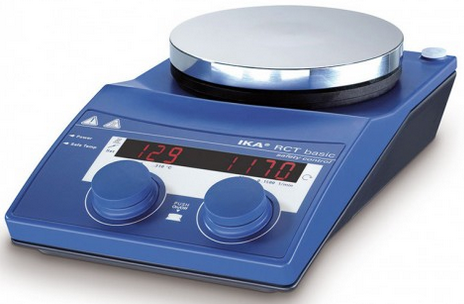
\includegraphics[width=0.44\textwidth]{Tarea1/basic.png}
        \caption{\textbf{RCT basic.}}
        \label{basic}
        \end{figure}
     \item \textbf{\textcolor{morado}{Thermo Scientific Multiskan GO}}: es un espectrofotómetro para microplacas, se utiliza para aplicaciones de investigación fotométrica, la cuantificación y pureza de ADN y ARN, ensayos con proteínas, ensayos con enzimas, ensayos cinéticos, inmunoensayos, ensayos de proliferación celular y citotoxicidad, ensayos de apoptosis, ensayos con gen indicador, ensayos GPCR.
     El mismo permite elegír realizar una libre elección de longitudes de onda de 200-1000 nm para las exigencias de diversos ensayos. Permite la lectura de microplacas y cubetas para las distintas demandas de productividad. Puede cambiarse el modo de muestreo a uno rápido de menos de 10 segundos o uno de alta calidad para un autodiagnóstico exhaustivo. % https://www.fishersci.es/shop/products/multiskan-go-microplate-spectrophotometer/p-4530546
        \begin{figure}
            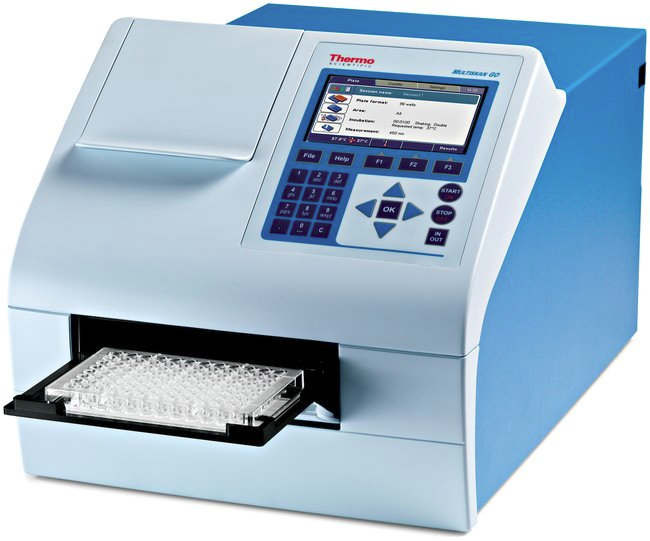
\includegraphics[width=0.44\textwidth]{Tarea1/espectro.png}
        \caption{\textbf{Thermo Scientific Multiskan.}}
        \label{espectro}
        \end{figure}
     \item \textbf{\textcolor{morado}{Pipetas para investigación}}: es necesaria para las tareas de pipeteo. La pipeta ultraligera cumple los más altos requisitos en cuanto a precisión y exactitud, ofreciendo a la vez una perfecta ergonomía así como una mayor flexibilidad. Se utilizarán pipetas de $20 - 200 ~\mu L$ y de $100 - 1000 ~\mu L$. Normalmente son ergonómicas. %http://www.labomersa.net/producto/pipetas-rresearch-plus/
        \begin{figure}
            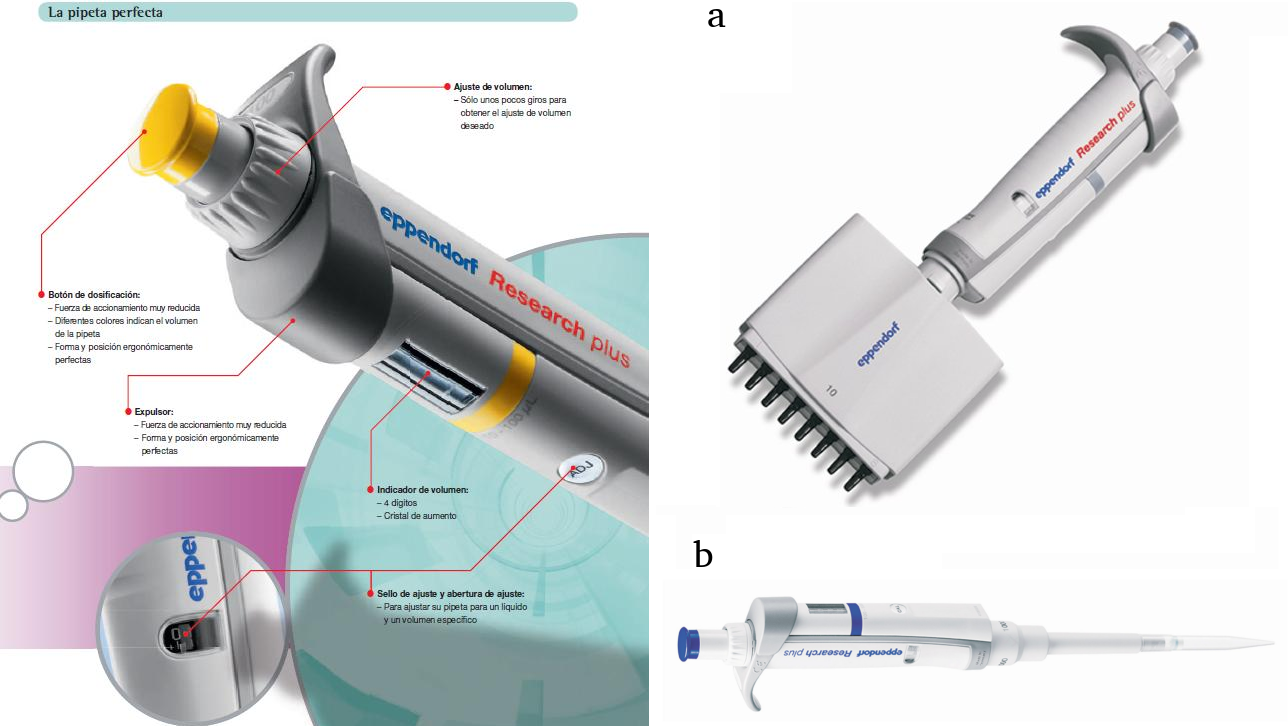
\includegraphics[width=0.44\textwidth]{Tarea1/pipeta.png}
            \caption{\textbf{Micropipetas Eppendorf Research Plus volumen variable, varios rangos}}
            \label{pipeta}
        \end{figure}
     \item \textbf{\textcolor{morado}{Thermo Scientific Heratherm IMC18 Incubator}}: es una incubadora microbiológica compacta . Tiene una capacidad de 18 litros y opera a temperatura de $17-40^oC$ en inferiores. Posee una uniformidad de temperatura de $\pm~ 1.2^oC$  y una estabilidad de temperatura de $\pm 0.2^oC$ (ambas medidas a $37^oC$), poseyendo por lo cual una alta exactitud de la temperatura.
        \begin{figure}
            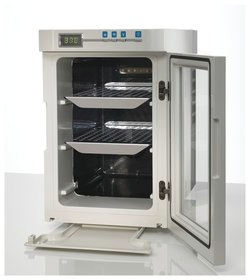
\includegraphics[width=0.4\textwidth]{Tarea1/incubadora.png}
        \caption{\textbf{Thermo Scientific Heratherm IMC18 Incubator.}}
        \label{incubadora}
        \end{figure}
        \item  \textbf{\textcolor{morado}{Nikon Inverted Microscope Eclipse Ti-U}}: es  un microscopio de investigación, el mismo es un modelo universal que puede configurarse para su uso con componentes motorizados adicionales que le permiten construir un microscopio para satisfacer muchas de las técnicas de microscopía más exigentes de la actualidad. El Eclipse Ti-U utiliza el mundialmente famoso sistema óptico CFI60 de Nikon y una amplia variedad de objetivos para las técnicas de microscopía de campo claro, campo oscuro, fluorescencia, contraste de fase, DIC y contraste de modulación.%http://www.einstmicroscopesolutions.com.sg/inverted-microscope-eclipse-ti-u/
        %https://www.microscope.healthcare.nikon.com/es_AMS/products/inverted-microscopes/eclipse-ti2-series
        \begin{figure}
            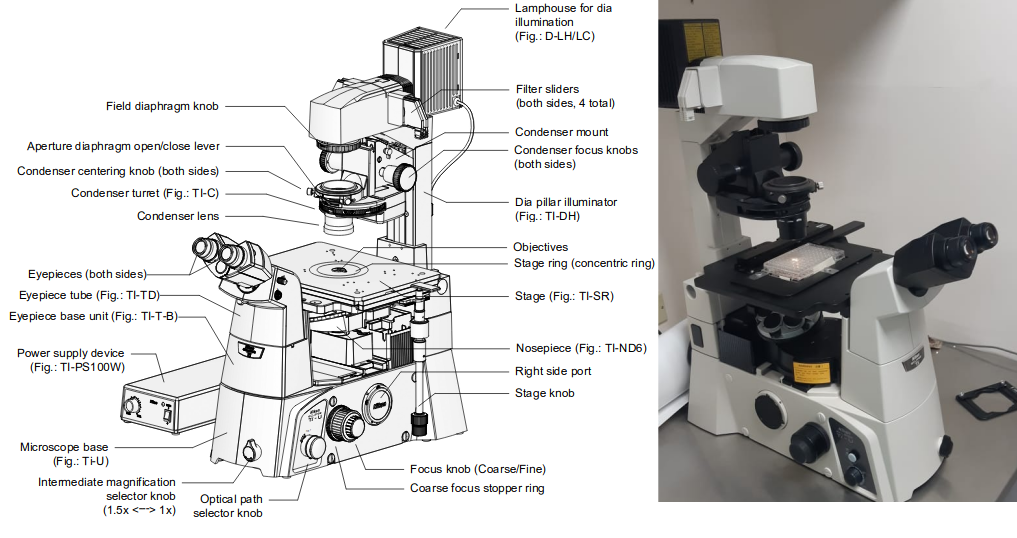
\includegraphics[width=0.4\textwidth]{Tarea1/microscopio.png}
        \caption{\textbf{ Nikon Inverted Microscope Eclipse Ti-U.}}
        \label{microscopio}
        \end{figure}
        \item \textbf{\textcolor{morado}{HI 2210 pH Meter Hanna}}: es un medidor de sobremesa de pH básico y económico que cuenta con calibración automática de 1 o 2 puntos con una selección de 5 memorias intermedias preprogramadas. Todas las lecturas se compensan automáticamente por las variaciones de temperatura de la sonda termistor suministrada. El medidor tiene una gran pantalla LCD fácil de leer que muestra el pH y la temperatura simultáneamente. %https://www.hannainst.es/parametros/4712-phmetro-sobremesa-basico-ph-temp-calibr-2-ptos.html
        \begin{figure}
            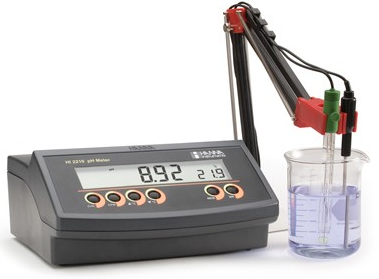
\includegraphics[width=0.4\textwidth]{Tarea1/ph.png}
        \caption{\textbf{ Nikon Inverted Microscope Eclipse Ti-U.}}
        \label{ph}
        \end{figure}
\end{itemize}
\textbf{\textcolor{azul50}{Conclusiones}}

 La primera práctica culmina con el recorrido del laboratorio y análisis del equipamiento que posteriormente se plantea trabajar. Se hace clara la necesidad de prudencia y organización en el trabajo en el laboratorio, ya que se presentan amenazas tanto para la salud individual como del equipo de trabajo, además se intenta proteger el equipamiento el cual puede sufrir daños como resultado de un mal manejo. 
 

 
 
 
 
 
 
 
 